
% The \phantomsection command is needed to create a link to a place in the document that is not a
% figure, equation, table, section, subsection, chapter, etc.
% https://tex.stackexchange.com/questions/44088/when-do-i-need-to-invoke-phantomsection
\phantomsection

% Multiple-language document - babel - selectlanguage vs begin/end{otherlanguage}
% https://tex.stackexchange.com/questions/36526/multiple-language-document-babel-selectlanguage-vs-begin-endotherlanguage
\begin{otherlanguage*}{brazil}

\chapter{Trabalhos Relacionados}

Neste capítulo, inicialmente é apresentado um artigo que descreve um modelo de plano de ensino baseado na plataforma Beecrowd, destacando suas justificativas e aspectos positivos. Em seguida, são analisados quatro artigos sobre a integração de diferentes ambientes de desenvolvimento com o Moodle: BOCA, CodeRunner, VPL, e um estudo sobre a integração de juízes online em geral com o Moodle. Por fim, são discutidos dois estudos focados na criação de sistemas especialistas web, explorando suas características e abordagens.

\section{Utilização da Plataforma Beecrowd de Maratona de Programação como Estratégia para o Ensino de Algoritmos}

Neste estudo conduzido por \cite{cruz2022}, é apresentada uma proposta de plano de ensino que se baseia no aproveitamento da plataforma Beecrowd para maratonas de programação, alinhada a abordagens pedagógicas ativas. Dessa maneira, são integrados conceitos como sala de aula invertida e gamificação, proporcionando uma abordagem dinâmica e envolvente no processo de aprendizagem e explorando as potencialidades da plataforma Beecrowd para oferecer uma experiência educacional inovadora. 

Os autores têm como objetivo aplicar essa metodologia de maneira a diminuir a curva de aprendizagem dos alunos, apoiar os professores na implementação de abordagens pedagógicas ativas em sala de aula e ampliar as oportunidades de interação entre os alunos, contribuindo assim para o desenvolvimento do aprendizado.

Os autores destacam a gamificação e a sala de aula invertida como estratégias que integram métodos de ensino com diversos recursos de comunicação, incluindo materiais escritos, orais e audiovisuais, junto a atividades, desafios e informações contextualizadas. A gamificação é apresentada como a aplicação de elementos característicos de jogos, uma abordagem eficaz para transformar a forma como os estímulos são apresentados aos alunos, visando engajá-los e incentivá-los a resolver problemas da maneira mais eficiente possível. 

De maneira semelhante, a sala de aula invertida é descrita como uma proposta para dinamizar a transmissão de informações durante as aulas, utilizando ferramentas online estruturadas e bem planejadas. Essa abordagem visa favorecer a iniciativa dos alunos ao estudarem previamente determinados conteúdos antes das aulas ministradas pelos professores.

Os autores ressaltaram a importância da disciplina de algoritmos como a base fundamental para o ensino de programação em diversos cursos na área da Informática. Essa disciplina aborda princípios essenciais de lógica de programação, visando desenvolver a capacidade dos estudantes em analisar e resolver problemas por meio da criação de algoritmos. Contudo, enfrenta desafios significativos, evidenciados pelo elevado índice de evasão e reprovação, tornando-se um ponto crítico nos cursos de graduação e impactando a continuidade dos alunos. 

A complexidade reside, em grande parte, na diversidade de alunos e em seus distintos estilos e ritmos de aprendizado, conforme indicado pelos autores. A adaptação eficiente a essa heterogeneidade representa um desafio no ensino de algoritmos e programação para novos estudantes. Nesse contexto, os autores propõem que a utilização de ferramentas online amplamente disponíveis para a aprendizagem ativa pode ser uma estratégia eficaz para permitir que cada aluno progrida em seu próprio ritmo e velocidade \cite[p.~5]{cruz2022}. 

No que diz respeito à integração de questões de maratonas de programação em sala de aula, os autores destacam sua relevância ao promover a busca ativa pela resolução de problemas. Ao buscar soluções, os alunos não apenas adquirem conhecimento sobre tópicos ainda não abordados em aula, mas também consolidam conceitos previamente ensinados.

O Beecrowd se destaca como uma ferramenta online que não apenas viabiliza a resolução de problemas em competições de programação, mas também se apresenta como uma valiosa aliada para o trabalho do professor. Os autores do estudo evidenciam que os desafios oferecidos pela plataforma Beecrowd estão meticulosamente organizados em categorias e níveis de dificuldade. As categorias abrangem temas como Iniciante, AD-HOC, Strings, Estruturas e Bibliotecas, Matemática, Paradigmas, Grafos, Geometria Computacional e SQL. A escala de dificuldade varia de 1 a 10, sendo 1 as questões mais acessíveis e 10 as mais desafiadoras.

No âmbito do artigo analisado, foram selecionadas questões da categoria Iniciante, e a partir delas, elaborou-se um plano de ensino voltado para a implementação da metodologia ativa da maratona de programação. Este plano foi aplicado em seis semestres na disciplina de algoritmos, envolvendo alunos que, em sua maioria, não possuíam conhecimento prévio em programação. A avaliação da proposta foi conduzida ao longo de três semestres que adotaram as metodologias ativas e outros três semestres que não as utilizaram, de forma intercalada. 

Através desse experimento e da análise de seus resultados, os autores constataram que a aplicação das metodologias de gamificação e sala de aula invertida contribuiu significativamente para o desempenho da turma, observando-se um crescimento notável. Além disso, as notas mais elevadas foram mais consistentes ao longo do tempo, demonstrando a eficácia dessas abordagens no contexto educacional.

Dessa forma, constatou-se que integrar o Beecrowd como um suporte para a implementação da gamificação como metodologia ativa na disciplina de algoritmos foi eficaz. A adoção do formato de maratona de programação possibilita ao professor envolver os alunos de forma mais imersiva, enquanto a plataforma oferece suporte adicional para o desenvolvimento da disciplina. Isso não apenas aprimora o processo de ensino e aprendizagem, mas também contribui para a redução da evasão em cursos superiores de informática.



\section{Integração do Ambiente BOCA com o Ambiente Moodle para Avaliação Automática de Algoritmos}

O estudo de \textcite{galasso} explora a integração entre o sistema BOCA \textit{Online Contest Administrator} e a plataforma Moodle, direcionada para o ensino de algoritmos. Essa integração visa proporcionar uma experiência simplificada para alunos e professores, facilitando o processo de avaliação automática de algoritmos no Moodle, já que o BOCA, além de gerenciar competições de programação, permitindo, assim, eventos como maratonas de programação, possui também um juiz automático para correção de algoritmos. Essa funcionalidade possibilita que os alunos recebam respostas imediatas sobre a correção de seus algoritmos, contribuindo para um aprendizado mais ágil e eficiente.

Na integração proposta, os professores podem criar questões de programação no Moodle, onde os alunos submetem códigos-fonte que são automaticamente avaliados pelo BOCA. Os algoritmos submetidos são compilados e executados com os dados de entrada predefinidos no Moodle, e suas saídas são comparadas com uma saída padrão para determinar se estão corretos. A resposta ao aluno é binária (correta ou incorreta), sem avaliação parcial, mas Moodle permite múltiplas tentativas, oferecendo a oportunidade de corrigir erros como problemas de compilação, formatação ou limite de tempo. Adicionalmente, o professor pode revisar manualmente os resultados, caso deseje realizar uma avaliação mais detalhada e parcial das respostas.

A figura 10 representa uma edição da tela de cadastro da questão, proporcionando uma visão ilustrativa desta fase do processo, já a figura 11 oferece uma representação visual da avaliação de uma questão como correta.

\begin{figure}[h!]
	   \centering
            \caption{Integração BOCA-Moodle - Edição de tela de cadastro de questão}
            \label{fig:ModeloConceitual}
	   	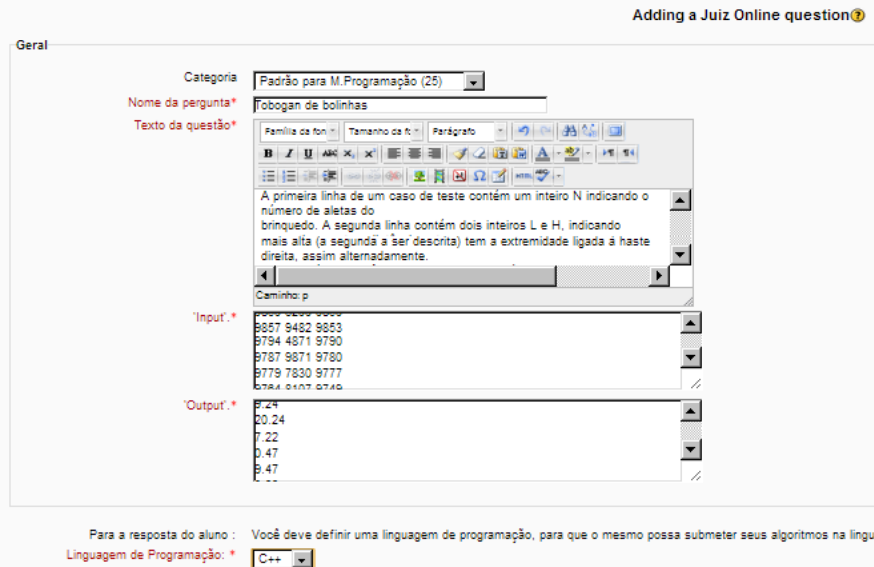
\includegraphics[scale=0.4]{pictures/BOCA_edicao.png}
        \fonte{\cite[p.~26]{galasso}}
\end{figure}

\begin{figure}[h!]
	   \centering
            \caption{Integração BOCA-Moodle - Visualização do retorno da avaliação da questão}
            \label{fig:ModeloConceitual}
	   	
\includegraphics[scale=0.4]{pictures/BOCA_visualizacao.png}
        \fonte{\cite[p.~27]{galasso}}
\end{figure}

Para manter o desempenho do Moodle, a integração foi concebida de modo a garantir que os ambientes envolvidos fossem implementados em servidores independentes. Essa separação minimiza a possibilidade de sobrecarga no Moodle durante a avaliação dos algoritmos no BOCA. A integração foi desenvolvida com o PostgreSQL, e os bancos de dados do Moodle e do BOCA se comunicam via Dblink, um recurso que permite o acesso remoto a tabelas específicas.

As tabelas principais do BOCA envolvidas na avaliação automática incluem a “problemtable”, para cadastro de questões, “runtable”, para submissões dos alunos, “answertable”, para dados de correção, e “langtable”, com as linguagens de programação suportadas (C, C++ e Java). Os autores também criaram duas tabelas auxiliares, “tempaluno” e “tempprofessor”, para facilitar a transferência de dados entre o Moodle e o BOCA.

Os gatilhos (triggers) configurados no banco de dados são fundamentais para o fluxo de dados entre Moodle e BOCA, eliminando a necessidade de alterações no código. O fluxo começa quando o professor cadastra uma questão no Moodle, acionando gatilhos que transferem os dados para o BOCA, onde a questão é registrada. Da mesma forma, quando um aluno responde, gatilhos adicionais transferem as submissões para a tabela de execução no BOCA.

\begin{figure}[h!]
	   \centering
            \caption{Integração BOCA-Moodle - Fluxo da interação das bases de dados do Moodle e do BOCA}
            \label{fig:ModeloConceitual}
	   	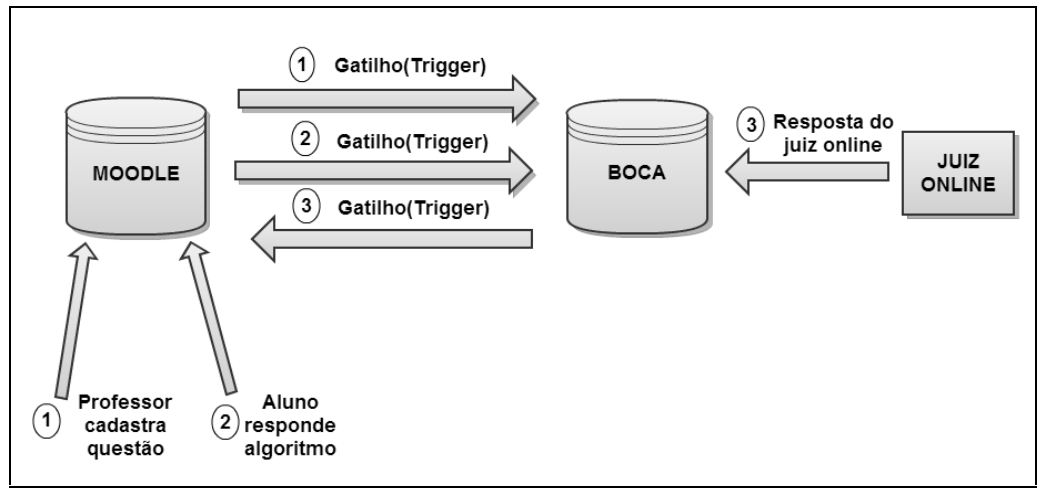
\includegraphics[scale=0.3]{pictures/BOCA_fluxo.png}
        \fonte{\cite[p.~29]{galasso}}
\end{figure}

Durante o julgamento das respostas, o BOCA executa scripts em intervalos de um minuto, verificando novas submissões e atualizando o status no Moodle. Os alunos visualizam uma área verde para respostas corretas e vermelha para incorretas. Figuras incluídas no estudo ilustram etapas do cadastro das questões e o \textit{feedback} visual ao aluno.

\begin{figure}[h!]
	   \centering
            \caption{Integração BOCA-Moodle - retorno da avaliação da questão como correta}
            \label{fig:ModeloConceitual}
	   	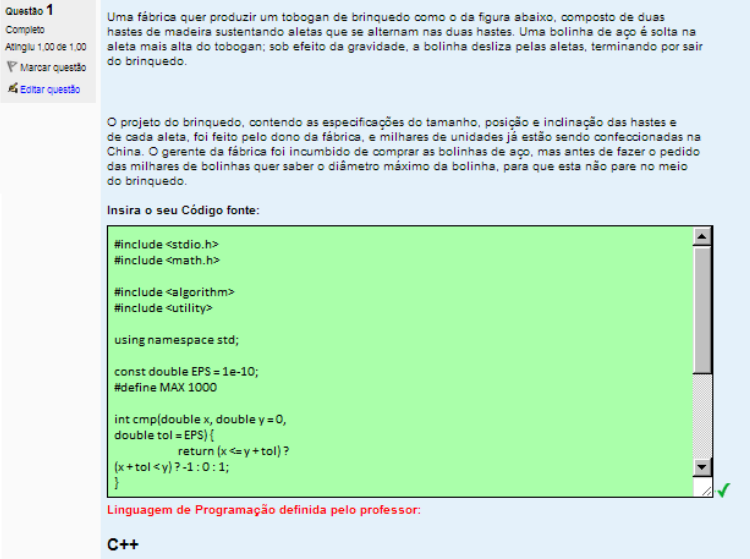
\includegraphics[scale=0.5]{pictures/BOCA_correta.png}
        \fonte{\cite[p.~26]{galasso}}
\end{figure}

Houve desafios técnicos, como a tentativa inicial de enviar arquivos “zip” diretamente para o banco de dados, o que levou a problemas de codificação. Para contornar isso, os arquivos foram transferidos via FTP, necessitando a instalação de um servidor FTP no ambiente do BOCA. Ao final, os autores ressaltam a importância de uma instalação simplificada e recomendam uma versão do BOCA já configurada para integração com o Moodle. Essa abordagem visa facilitar a adoção da solução e sua eficácia no ensino de algoritmos.

\section{CodeRunner: A Tool for Assessing Computer Programing Skills}

O estudo de \textcite{lobbharlow} examina as dificuldades encontradas na avaliação de alunos em disciplinas de programação utilizando métodos tradicionais, como provas de papel e caneta. O artigo destaca que a complexidade dos códigos e a natureza da programação moderna tornam a avaliação precisa um desafio, pois esses métodos não oferecem a possibilidade de realizar testes ou debug. O artigo propõe o uso de ferramentas de avaliação automatizadas, como o CodeRunner, que proporciona correção e \textit{feedback} imediato para os alunos.	

Pelo CodeRunner, plugin do Moodle, os alunos recebem um \textit{feedback} binário, onde as respostas corretas são indicadas por marcas verdes e as incorretas por cruzes vermelhas. A ferramenta adota o método de avaliação "tudo ou nada", ou seja, uma resposta só é considerada correta se atender completamente aos requisitos do teste, sendo a nota zero atribuída para respostas incorretas. Contudo, o sistema permite que os alunos façam múltiplas tentativas, oferecendo a chance de corrigir falhas como erros de compilação, formatação inadequada ou problemas de tempo de execução, com a possibilidade de aplicar penalidades em caso de envio tardio ou repetido.

\begin{figure}[h!]
	   \centering
            \caption{CodeRunner - A simples pergunta sobre Python, respondida erroneamente}
            \label{fig:ModeloConceitual}
	   	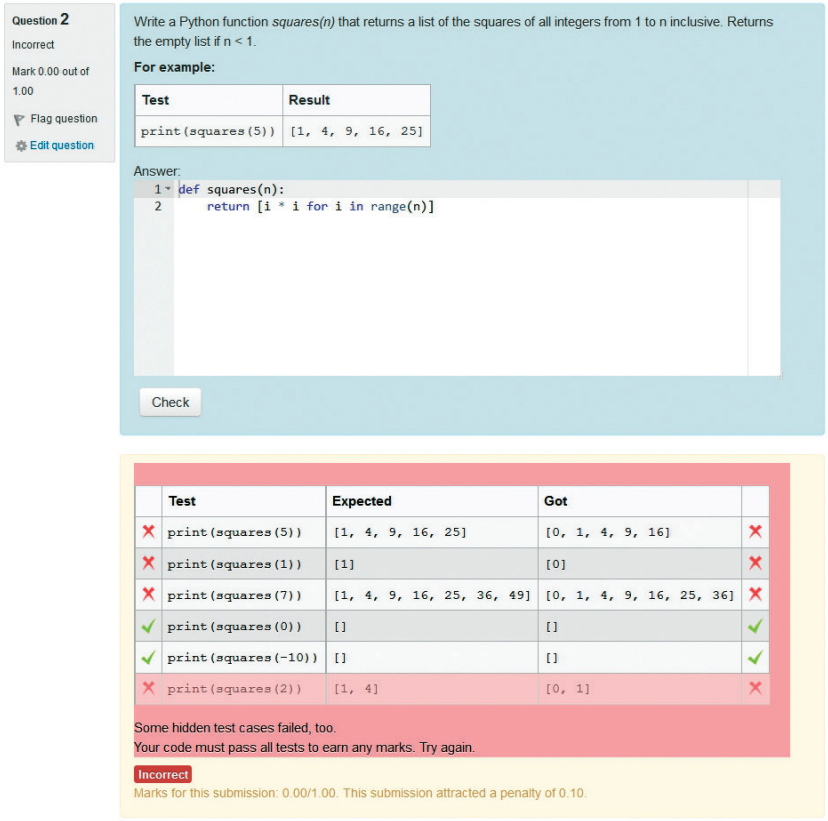
\includegraphics[scale=0.4]{pictures/CodeRunner_errada.png}
        \fonte{\cite[p.~48]{lobbharlow}}
\end{figure}

\begin{figure}[h!]
	   \centering
            \caption{CodeRunner - A simples pergunta sobre Python, respondida corretamente}
            \label{fig:ModeloConceitual}
	   	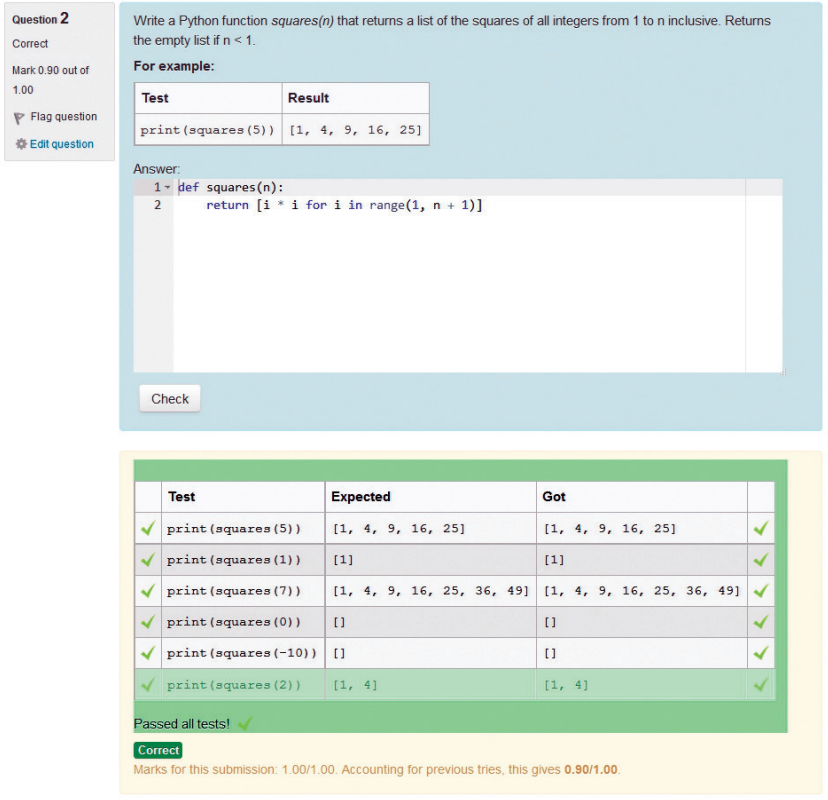
\includegraphics[scale=0.4]{pictures/CodeRunner_correta.png}
        \fonte{\cite[p.~48]{lobbharlow}}
\end{figure}

O CodeRunner também apresenta uma abordagem flexível para a criação de perguntas, permitindo que os desenvolvedores de questões criem protótipos personalizados. Esses protótipos podem ser usados para perguntas que exigem funcionalidades adicionais ou para impor restrições, como o uso de determinado tipo de estrutura de controle no código. Além disso, a execução do código do aluno ocorre em um ambiente seguro, isolado do servidor principal, o que evita riscos de segurança.

Apesar de o CodeRunner ter se revelado altamente eficaz em diversas atividades de avaliação, os autores destacaram algumas limitações fundamentais:

\begin{enumerate} [label=(\alph*)]
    \item O CodeRunner destaca-se em tarefas relativamente simples com especificações claras. Embora, teoricamente, qualquer pergunta com resposta mensurável por um programa de computador possa ser formulada como uma pergunta do CodeRunner, o esforço demandado para criar avaliadores para tarefas complexas muitas vezes inviabiliza essa abordagem, especialmente em turmas de maior tamanho;
    \item Ferramentas de qualidade de código, como o pylint, provaram ser muito valiosas para aumentar a conscientização sobre o estilo e melhorar a qualidade do código, mas ainda ocorrem abusos das regras de estilo, e a qualidade dos comentários e identificadores não pode ser avaliada por computador. Por isso, a avaliação humana ainda é reservada para a qualidade do código;
    \item A resposta a uma pergunta do CodeRunner deve ser apresentada como um único bloco de texto, predominantemente composto por código. Embora os autores das perguntas possam gerar diversos formatos de \textit{feedback}, inclusive gráficos, a apresentação padrão dos resultados é tabular, com uma linha para cada caso de teste e correspondência direta entre a saída esperada e a saída real. Caso os testes exijam blocos extensos de código ou resultem em saídas volumosas, a visualização dos resultados pode dificultar a compreensão pelos alunos do motivo pelo qual uma resposta foi marcada como incorreta;
    \item A avaliação de perguntas com resultados gráficos representa um desafio. Foi criado uma simulação do kit de ferramentas GUI tkinter em Python para avaliar interfaces gráficas na disciplina, incluindo perguntas que verificam a precisão de gráficos gerados por chamadas à biblioteca de gráficos do Matlab. Contudo, a avaliação da correção de imagens ou mesmo da saída de programas que envolvem gráficos complexos, como os da biblioteca de tartarugas, foi considerada uma tarefa difícil, senão impossível;
    \item Por último, é importante ressaltar que a elaboração de perguntas de qualidade e testes eficazes pode demandar considerável tempo, mesmo em cursos de programação de nível básico. O compartilhamento de bancos de dados de perguntas entre professores seria altamente benéfico nesse contexto.
\end{enumerate}


\section{A Virtual Programming Lab for Moodle with Automatic Assessment and Anti-Plagiarism Features}

\textcite{rodriguezdelpinoandroyo} descreveram neste artigo o módulo Virtual Programming Lab (VPL) para o Moodle, desenvolvido na Universidade de Las Palmas de Gran Canaria (ULPGC), e lançado para uso gratuito sob a licença GNU/GPL.

Para empregar uma linguagem de programação específica no VPL, basta garantir que o compilador correspondente esteja devidamente instalado no sistema de execução. Atualmente, estão disponíveis sistemas de execução com instalações para diversas linguagens, incluindo Ada, C, C\+\+, C\#, FORTRAN, Haskell, Java, Octave, Pascal, Perl, PHP, Prolog, Python, Ruby, Scheme, SQL e VHDL.
 
O VPL é composto por três elementos: um módulo do Moodle, um editor de código baseado em navegador e um componente Jail, mostrados na figura 16.

\begin{figure}[h!]
	   \centering
            \caption{VPL - Componentes}
            \label{fig:ModeloConceitual}
	   	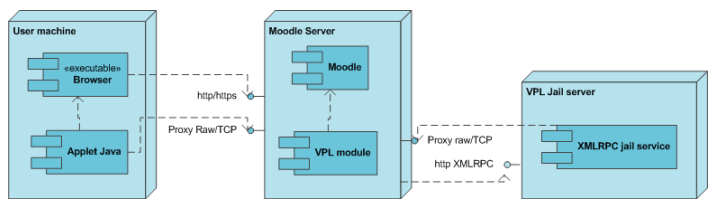
\includegraphics[scale=0.5]{pictures/VPL_componentes.png}
        \fonte{\cite[p.~2]{rodriguezdelpinoandroyo}}
\end{figure}

O editor de código, construído em Java, possibilita a edição, execução, depuração e avaliação de programas em um ambiente simples de desenvolvimento. Já o módulo do Moodle oferece características típicas, como backup, integração com o livro de notas e controle de eventos, além de recursos específicos, como gerenciamento de submissões, suporte à avaliação e prevenção contra plágio. E o componente Jail é um servidor que compila e executa códigos de alunos em um ambiente seguro, usando o comando linux chroot para restrições de leitura. 

O VPL permite configurar, gerenciar e avaliar atividades de aprendizagem, classificadas por tipo (exemplos, exercícios de cloze, exercícios de desenvolvimento de código) e escopo (tarefas fora da sala de aula ou exames em sala).

A criação de uma atividade VPL inicia-se com o preenchimento do formulário de configuração básica no Moodle, incluindo nome, descrição, período de disponibilidade, opções de avaliação e outras configurações. Além disso, é possível especificar detalhes como número máximo de arquivos, tamanho máximo, restrições de edição, rede e senha. Veja na imagem 18.

\begin{figure}[h!]
	   \centering
            \caption{VPL - Configuração básica de restrições}
            \label{fig:ModeloConceitual}
	   	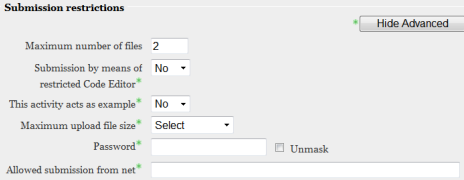
\includegraphics[scale=0.5]{pictures/VPL_config_basica.png}
        \fonte{\cite[p.~3]{rodriguezdelpinoandroyo}}
\end{figure}

Após preencher o formulário básico, o instrutor pode ajustar cinco grupos adicionais de recursos na ferramenta VPL. A guia "Descrição completa" permite fornecer detalhes sobre o problema a ser resolvido. Em "Casos de teste", é possível configurar testes com descrição, entrada, saída esperada e penalizações em caso de falha. A guia "Options" configura aspectos gerais, como a base da atividade, permissões dos alunos e se os resultados automáticos contam para a nota final. "Arquivos solicitados" determina os nomes obrigatórios dos arquivos a serem enviados. 

Essas configurações são suficientes, mas a guia "Advanced" oferece recursos adicionais para testes mais elaborados, como testes de funcionalidade avançados e outros tipos de teste, possibilitando uma avaliação abrangente da qualidade do código.

A figura 19 mostra um exemplo de configuração de casos de teste, e a figura 20 mostra a tela de configuração de casos de teste mais avançados.

\begin{figure}[h!]
	   \centering
            \caption{VPL - Exemplo de configuração de casos de teste}
            \label{fig:ModeloConceitual}
	   	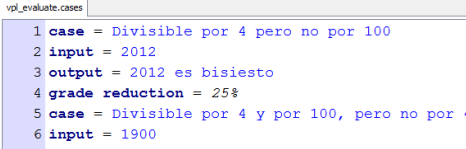
\includegraphics[scale=0.5]{pictures/VPL_testes.png}
        \fonte{\cite[p.~3]{rodriguezdelpinoandroyo}}
\end{figure}

\begin{figure}[h!]
	   \centering
            \caption{VPL - Arquivos de execução para testes avançados}
            \label{fig:ModeloConceitual}
	   	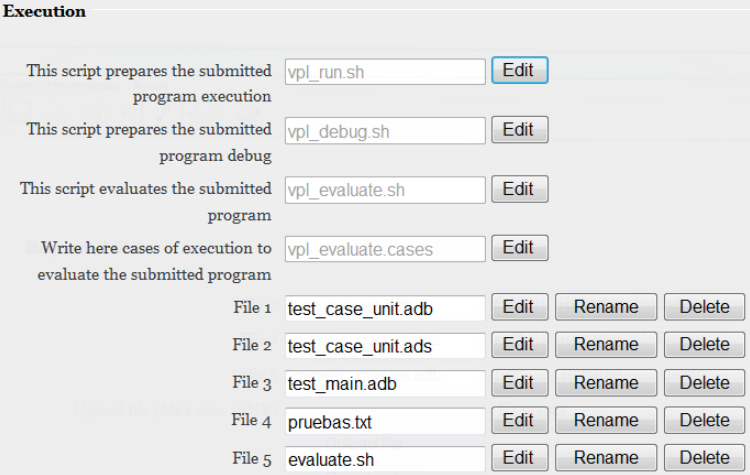
\includegraphics[scale=0.5]{pictures/VPL_testes_avancados.png}
        \fonte{\cite[p.~4]{rodriguezdelpinoandroyo}}
\end{figure}

O VPL oferece avaliação automática e assistida por computador, permitindo a personalização através das opções na guia correspondente. É essencial configurar os testes para respaldar a avaliação. O VPL realiza automaticamente os testes configurados, fornecendo um relatório com testes falhos, comentários explicativos e uma proposta de nota. O avaliador humano tem a flexibilidade de ajustar o relatório, excluindo ou adicionando comentários, reutilizando itens da lista e recalculando a nota conforme necessário.

O plágio é abordado pelo VPL através de uma ferramenta de verificação de plágio no código-fonte. Essa ferramenta procura identificar plágio entre os envios de uma tarefa em um curso, considerando também fontes como envios anteriores ou tarefas similares de outros cursos. O processo de identificação de semelhanças entre os arquivos de origem envolve três etapas: tokenização, comparação e clusterização. 

A tokenização visa obter uma assinatura normalizada para facilitar a comparação eficiente, envolvendo análise lexical, filtragem e normalização. Esse processo cria uma assinatura do programa, que é uma representação normalizada dos arquivos de código-fonte de um usuário, otimizando o processo de comparação, permitindo a detecção eficaz de plágio.

Em resumo, o Virtual Programming Lab (VPL) apresenta-se como uma ferramenta abrangente para o gerenciamento de atividades de programação. Com recursos que vão desde a configuração detalhada de atividades no Moodle até a execução de testes avançados e a detecção de plágio, o VPL oferece uma variedade de funcionalidades para apoiar a aprendizagem prática e avaliação de habilidades de programação. Destaca-se, além disso, a necessidade de configurar todos os exercícios e seus casos de teste, para disponibilização destes aos alunos.


\section{Uma Ferramenta Baseada em Juízes Online para o Apoio às Atividades de Programação de Computadores no Moodle}

No projeto conduzido por \textcite{joseosvaldochaves}, foi desenvolvido o Módulo de Integração com Juízes Online (MOJO), ferramenta que integra os Juízes Online, como o Timus Online Judge e o Beecrowd (conhecido como URI Online Judge na época) ao Moodle, para evitar que os professores de disciplinas de programação ficassem sobrecarregados ao ter que elaborar, submeter, abaliar e fornecer o \textit{feedback} necessário das questões aos alunos. O MOJO automatizou o processo de Elaboração, Submissão e Avaliação (ESA) das atividades de programação, fornecendo um ambiente unificado que facilita o acompanhamento dos alunos e amplia o acesso a um maior número de questões.

O MOJO, portanto, integra o Moodle com os Juízes Online para atividades de programação, sem interação direta entre as plataformas. Ele automatiza o processo ESA (Elaboração, Submissão e Avaliação), permitindo que professores submetam questões no Moodle, estudantes enviem suas respostas, e os Juízes Online avaliem automaticamente o código, com os resultados retornando ao Moodle para análise de professores e alunos. O professor pode monitorar o progresso dos estudantes e acessar os códigos submetidos, enquanto o Repositório de Integração armazena as questões para uso futuro.

Na arquitetura geral do MOJO, o Moodle gerencia a interface e o controle das atividades de programação, enquanto o MOJO se encarrega da comunicação e interação com os Juízes Online. A arquitetura conta com o Módulo Principal (MOP), responsável pelas funcionalidades essenciais e pelo controle do Módulo de Carga e Atualização (MOCA), que, por sua vez, realiza o carregamento inicial e atualizações constantes das questões, armazenando-as no Repositório de Integração. Esse repositório mantém as questões e resultados para uso e acompanhamento contínuo no Moodle.

Como os juízes online não oferecem APIs ou serviços Web, foram necessárias implementações específicas para cada juiz, utilizando PHP (a mesma linguagem do Moodle) e JavaScript para a interface. O banco de dados PostgreSQL foi escolhido por ser open-source e por permitir a criação de tabelas personalizadas para armazenar dados dos alunos, viabilizando um \textit{feedback} direcionado e adequado.

O objetivo do MOJO é reduzir a carga de trabalho dos professores no processo ESA, permitindo um acompanhamento mais próximo dos alunos. Em uma pesquisa inicial com sete professores, os resultados apontaram que 71,4\% acreditam que a ferramenta pode economizar tempo; 28,6\% gostariam de poder criar e avaliar suas próprias atividades automaticamente; 42,8\% mencionaram questões de legibilidade do código; 28,6\% observaram a clareza dos resultados; 85,7\% valorizam o \textit{feedback} mais rápido aos alunos; e 100\% acreditam que a redução de tarefas possibilitará um acompanhamento mais eficaz, especialmente para alunos com dificuldades.


\section{Building of a Rule-Based Expert System for Academic Advising via Web Expert System Tools}

O projeto conduzido por \textcite{osmannasr} aborda o desenvolvimento de um sistema especialista voltado para otimizar o aconselhamento acadêmico na Universidade King Khalid. A proposta central do estudo é criar uma ferramenta que simule as funções do conselheiro acadêmico humano, utilizando técnicas de inteligência empresarial para auxiliar na tomada de decisões informadas por estudantes e funcionários, baseadas nas regulamentações acadêmicas da instituição.

O processo de desenvolvimento do sistema é dividido em várias fases, cada uma com objetivos específicos:

Fase de Análise: Esta etapa inicial é dedicada à coleta de informações sobre as questões mais recorrentes entre os estudantes, além de procedimentos acadêmicos frequentes, como matrícula em cursos, transferências de departamento e pedidos de suspensão. A análise dessas necessidades foi realizada por meio de entrevistas com estudantes e conselheiros acadêmicos, utilizando uma abordagem de árvore de decisão (UML), mostrada na Figura 20, para entender melhor os requisitos do sistema.

\begin{figure}[h!]
        \centering
         \caption{Sistema especialista baseado em regras - Árvore de decisão}
         \label{fig:ModeloConceitual}
                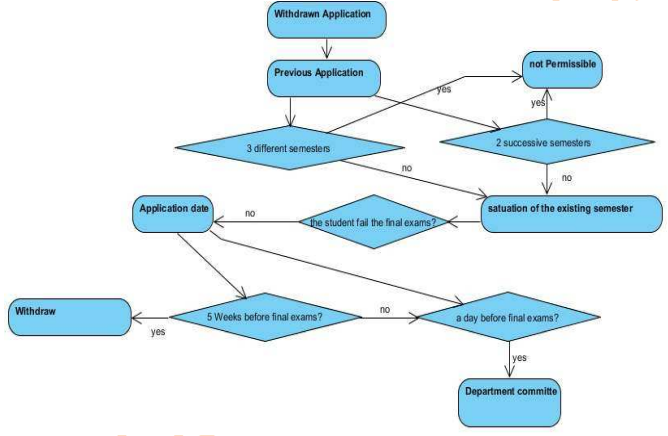
\includegraphics[scale=0.5]{pictures/Rule_Based_Expert_System_arvore_decisao.png}
     \fonte{\cite{osmannasr}}
\end{figure}

Fase de Design: Com base na análise anterior, o design do sistema foi estruturado utilizando uma metodologia baseada em regras (rule-based). Esse método foi escolhido por sua adequação à modelagem dos processos de aconselhamento acadêmico, que envolvem uma lógica condicional do tipo "se-então". Durante essa fase, também foi projetada uma interface amigável, alinhada com o estilo visual e os padrões de interação do portal da universidade, garantindo que os usuários pudessem facilmente se adaptar ao sistema.

Fase de Implementação: A construção do sistema foi realizada utilizando o ES Builder, uma ferramenta de código aberto que facilita a criação de sistemas especialistas baseados em regras. O sistema foi projetado para ser acessível via plataforma web, o que possibilita seu uso por uma grande variedade de usuários, incluindo estudantes e conselheiros acadêmicos.

Fase de Testes e Avaliação: O sistema foi testado com diferentes cenários, utilizando tanto estudantes quanto conselheiros acadêmicos, a fim de validar sua eficácia. Os resultados indicaram que o sistema é capaz de fornecer respostas adequadas e de auxiliar no processo de aconselhamento de forma precisa e eficiente.

O estudo conclui que a implementação de sistemas especialistas no âmbito acadêmico tem um grande potencial para melhorar a eficiência do aconselhamento acadêmico, promovendo uma interação mais eficaz entre estudantes e conselheiros. Além disso, o sistema proposto pode se tornar uma ferramenta valiosa para a tomada de decisões informadas, não apenas para os estudantes, mas também para os docentes, que poderão fornecer orientações mais precisas e baseadas em dados. O sistema mostrou-se alinhado às expectativas dos usuários, que manifestaram interesse em expandir sua funcionalidade para cobrir mais áreas do aconselhamento acadêmico.

Este trabalho evidencia o papel transformador que a tecnologia pode desempenhar no setor educacional, especialmente no contexto do aconselhamento acadêmico, apontando para a necessidade de continuar a pesquisa e o desenvolvimento de sistemas dessa natureza para atender de forma mais abrangente às necessidades dos estudantes e professores.


\section{An Interactive Web-Based Expert System Degree Planner}

O artigo desenvolvido por \textcite{neildunstan} descreve o desenvolvimento de um planejador de grau acadêmico baseado na web (seu layout é mostrado na Figura 21), utilizando XML (Extensible Markup Language) e sistemas especialistas. O sistema possui um servidor que hospeda arquivos XML para cada grau acadêmico, descrevendo unidades e regras associadas. Essas regras são importadas para uma interface web genérica, permitindo a personalização do visual com uma paleta de unidades e horários disponíveis para os semestres. As regras do grau acadêmico em formato XML são convertidas em código Prolog, que permite ao sistema responder a consultas complexas relacionadas ao planejamento de cursos.

\begin{figure}[h!]
        \centering
         \caption{Planejador de grau acadêmico - Layout da página}
         \label{fig:ModeloConceitual}
                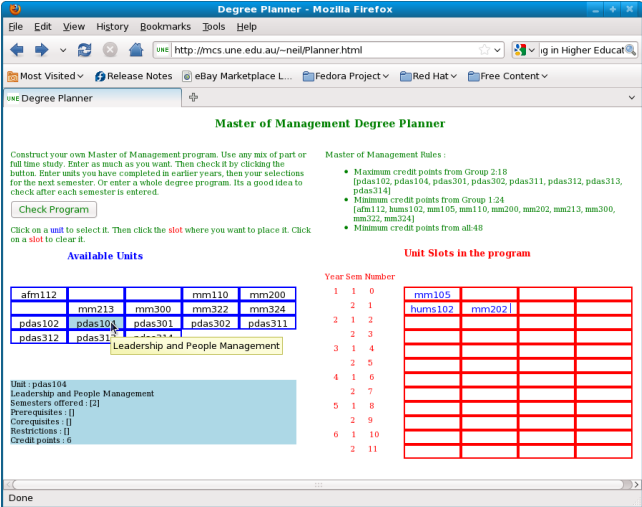
\includegraphics[scale=0.5]{pictures/degree_planner_page_layout.png}
     \fonte{\cite{neildunstan}}
\end{figure}

O design do sistema é baseado na separação clara entre o tratamento da interface do usuário no cliente e o processamento de regras no servidor (Figura 22). O servidor utiliza um sistema especialista em Prolog para resolver consultas mais complexas, enquanto o cliente lida com informações mais simples por meio de JavaScript. O sistema é acessível via navegador e não requer plugins específicos, sendo adequado para dispositivos móveis, como smartphones.

\begin{figure}[h!]
        \centering
         \caption{Planejador de grau acadêmico - Interação cliente-servidor}
         \label{fig:ModeloConceitual}
                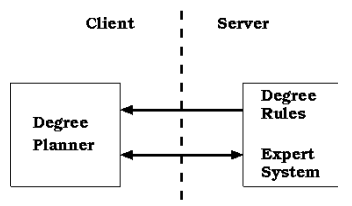
\includegraphics[scale=0.5]{pictures/degree_planner_client_server.png}
     \fonte{\cite{neildunstan}}
\end{figure}

A interface do usuário é composta por várias seções, incluindo uma paleta de unidades, um cronograma de programa semestral e um painel de exibição de detalhes das unidades selecionadas. Os estudantes podem explorar opções de inscrição e verificar se suas escolhas atendem aos requisitos do curso. O sistema permite que os alunos ajustem seu programa acadêmico, respondendo a perguntas sobre requisitos de unidades e pré-requisitos, de forma interativa e personalizada.

Conclui-se que o uso de sistemas especialistas em planejadores de grau acadêmico baseados na web pode melhorar a interatividade e fornecer orientações mais precisas aos alunos, ajudando-os a construir um programa de graduação adequado aos seus interesses e cronograma, sem a necessidade de plugins ou instalações específicas.


\section{Comparação entre os Trabalhos}

O estudo de \cite{cruz2022} ressalta a eficácia da integração da plataforma Beecrowd em um plano de ensino inovador para disciplinas de programação. Ao incorporar estratégias como sala de aula invertida e gamificação, a pesquisa conclui que o Beecrowd, utilizado como suporte para a gamificação, não só melhora o processo de ensino e aprendizagem, oferecendo suporte aos educadores e motivando os alunos, mas também contribui para a redução da evasão em cursos superiores de informática.

A aplicação das metodologias propostas no estudo dos autores demonstrou um impacto significativo no desempenho dos alunos ao longo do tempo na universidade dos autores, resultando em um crescimento notável e consistente nas notas. A ferramenta Beecrowd, destacada no estudo, é elogiada pela sua organização meticulosa de desafios em categorias e níveis de dificuldade, além de sua abordagem de maratona de programação, revelando-se eficaz em envolver os alunos de maneira imersiva.

A Tabela 1 apresenta uma comparação detalhada das vantagens do Beecrowd em relação a outras ferramentas integradas ao Moodle, como BOCA, VPL e CodeRunner, conforme discutido nos trabalhos relacionados. O objetivo é analisar os benefícios específicos do uso do Beecrowd, oferecendo uma base sólida para este estudo. Vale ressaltar que este trabalho propõe o incentivo ao uso da integração entre Moodle e Beecrowd por meio de LTI. Em contraste, o BOCA e o CodeRunner funcionam como tipos de questões no Moodle, enquanto o VPL é um módulo próprio da plataforma.

\begin{table}[htb]
        \IBGEtab{%
          \caption[Comparação entre quatro integrações de sistemas, que auxiliam no ensino da programação, com o Moodle: Beecrowd, BOCA, CodeRunner e VPL]{Comparação entre quatro integrações de sistemas, que auxiliam no ensino da programação, com o Moodle: Beecrowd, BOCA, CodeRunner e VPL}%
          \label{tabela-ibge}
        }{%
          \begin{tabular}{c c c c c}
          \toprule
           \textbf{Aspecto} & \textbf{Beecrowd} & \textbf{BOCA} & \textbf{VPL} & \textbf{CodeRunner} \\
          \midrule
          Possui Juiz Online	                        &  X	& X	& X	& X   \\ \midrule
          Fornece \textit{feedback} Imediato	                &  X	& X	& X	& X   \\ \midrule
          Criação Manual de Questões	                &  	& X	& X	& X   \\ \midrule
          Questões Prontas para Professores	        &  X	& 	& 	&    \\ \midrule
          Questões Prontas classificadas por categoria  &  X	& 	& 	&    \\ \midrule
          Inserção Manual de Casos de Teste	        &  	& X	& X	& X   \\ \midrule
          Suporta Diversas Linguagens	                &  X	& X	& X	& X   \\ \midrule
          Pré-processamento de Submissões	        &  	& 	& 	& X   \\ \midrule
          Comentários de Testes Falhados	        &  	& 	& X	&    \\ \midrule
          Prevenção de Plágio	                        &  X	& 	& X	&    \\ \midrule
          Incentiva participar de maratonas de programação    &  X	& 	& 	&    \\ 
          \bottomrule
        \end{tabular}%
        }{%
          \fonte{
              Produzido pela autora. 
          }%
        }
      \end{table}

A análise da tabela destaca o Beecrowd como notavelmente diferenciado em relação aos outros sistemas, sobretudo devido à presença de questões pré-existentes para os professores. Essa característica elimina a necessidade de cadastramento manual das questões de programação e seus respectivos testes, uma exigência presente nas plataformas BOCA, VPL e CodeRunner. Como confirmação, uma das limitações do CodeRunner apontadas por \textcite{lobbharlow} é o fato de a criação de perguntas e testes de qualidade demandar tempo, além de ser mais adequado para tarefas simples e bem definidas, já que a criação de testes para atividades complexas exige muito esforço, especialmente em turmas grandes.

Um aspecto distintivo e relevante nos sistemas BOCA, VPL e CodeRunner é a abordagem de desenvolvimento que incorpora a utilização de servidores separados para o Moodle e os sistemas juízes online. Essa estratégia visa garantir a execução independente e eficiente de cada componente, proporcionando benefícios tanto em termos de desempenho quanto de segurança.

A adoção de servidores separados para o Moodle e os sistemas juízes online tem como objetivo otimizar a distribuição de carga, prevenindo sobrecargas e garantindo uma operação mais estável e responsiva. Essa separação também fortalece a segurança, pois ao isolar cada plataforma, diminui-se os riscos de conflitos e vulnerabilidades. Da mesma forma, ela possibilita uma escalabilidade mais eficiente, permitindo que cada sistema seja dimensionado conforme suas necessidades específicas, sem afetar o desempenho do outro. Isso é particularmente importante em ambientes acadêmicos, onde a demanda por plataformas e sistemas pode variar significativamente.

O trabalho de \textcite{rodriguezdelpinoandroyo} mostra que o módulo Virtual Programming Lab (VPL) possui um editor de código em Java para editar, executar, depurar e avaliar programas em um ambiente simples de desenvolvimento. Dessa forma, para utilizar todas as funcionalidades é necessário um navegador com suporte a JavaScript e applets Java. Já os trabalhos de \textcite{lobbharlow} e \textcite{galasso} mostram que tanto o CodeRunner quanto o BOCA disponibilizam caixas de texto nas quais os usuários podem escrever ou colar o código, permitindo sua subsequente avaliação.

Neste trabalho, a integração LTI fornecida pelo Beecrowd será utilizada, de modo que a criação de listas de exercícios, a resolução de exercícios pelos alunos e a correção das soluções pelo juiz online ocorrerão diretamente nos servidores do Beecrowd.

Além disso, a prevenção contra plágio é uma característica crucial e distintiva tanto no Beecrowd quanto no VPL, destacando-se como um diferencial significativo dessas plataformas. Essa funcionalidade visa salvaguardar a integridade acadêmica, garantindo que os trabalhos submetidos pelos alunos sejam autênticos e originais.

No contexto do Beecrowd, de acordo com \cite{cruz2022}, a prevenção contra plágio pode envolver mecanismos avançados de análise de código-fonte, identificando padrões suspeitos que indicam possível cópia indevida. Além disso, o sistema pode empregar algoritmos e técnicas que comparam soluções de diferentes alunos, buscando similaridades que ultrapassem limites aceitáveis de coincidência.

No caso do VPL, de acordo com \textcite{rodriguezdelpinoandroyo}, a prevenção contra plágio pode ser implementada através de verificações rigorosas durante o processo de submissão. Isso pode incluir a comparação automática de códigos submetidos em busca de trechos idênticos ou substancialmente semelhantes. Além disso, o VPL pode adotar métodos de análise mais avançados, como a detecção de técnicas de programação específicas que são características de trabalhos plagiados.

O projeto de \textcite{joseosvaldochaves} descreve o desenvolvimento do Módulo de Integração com Juízes Online (MOJO), uma ferramenta criada para integrar juízes online, como o Beecrowd (anteriormente URI Online Judge), ao Moodle. O MOJO visa delegar ao Moodle o gerenciamento da interface e do controle das atividades de programação, enquanto centraliza a comunicação e interação com os juízes online. Devido à ausência de APIs ou serviços web nos juízes à época, foram necessárias implementações específicas para cada plataforma, utilizando PHP (a mesma linguagem do Moodle) e JavaScript para a interface. O banco de dados PostgreSQL foi adotado por ser open-source e pela flexibilidade de criação de tabelas personalizadas para armazenamento de dados dos alunos, o que possibilita um \textit{feedback} direcionado e preciso.

Este trabalho, contudo, utilizará a integração LTI fornecida pelo Beecrowd, a qual facilita a interação de docentes e alunos com a plataforma. Além disso, será disponibilizado um manual para orientar o uso da LTI, juntamente com um sistema especialista que auxiliará os alunos na resolução das questões e os docentes no esclarecimento de dúvidas dos estudantes.

É relevante notar que 100\% dos professores entrevistados para avaliar a eficácia do MOJO acreditam que a redução de tarefas permitirá um acompanhamento mais eficaz dos estudantes, especialmente daqueles que apresentam maiores dificuldades.

Por fim, os projetos de \textcite{osmannasr} e \textcite{neildunstan} abordam a construção de sistemas especialistas para o aconselhamento e planejamento acadêmico, porém apresentam enfoques e abordagens técnicas distintas.

No primeiro trabalho, \textcite{osmannasr} desenvolve um sistema especialista baseado em regras para o aconselhamento acadêmico na Universidade King Khalid. Este sistema é focado em replicar o processo de tomada de decisão dos conselheiros acadêmicos humanos, utilizando uma metodologia de árvore de decisão, implementada através do ES Builder, uma ferramenta de código aberto para sistemas especialistas baseados em regras, com uma interface web simples e uma lógica de "se-então". Essa escolha reflete a necessidade de simular de forma prática e direta o trabalho dos conselheiros humanos sem uma complexidade computacional elevada.

No segundo trabalho, \textcite{neildunstan} foca em um planejador de grau acadêmico, utilizando uma abordagem híbrida com XML e Prolog para gerenciar e responder a consultas complexas. As regras para cada programa acadêmico são estruturadas em XML e convertidas em Prolog, possibilitando que o sistema lide com consultas interativas e personalizadas. A arquitetura desse sistema é distribuída, com o cliente manipulando a interface e o servidor processando as regras em Prolog. Essa separação facilita o uso em dispositivos móveis e oferece flexibilidade ao permitir que os alunos construam e verifiquem seu programa acadêmico de maneira independente e intuitiva, sem plugins específicos.

Já neste trabalho, será utilizado o Prolog como servidor da aplicação, responsável pelo gerenciamento de requisições HTTP, armazenamento de dados de sessão e comunicação contínua com o front-end. O servidor proporcionará um ambiente dinâmico para o carregamento modular de arquivos específicos de cada questão, permitindo a adaptação das perguntas e a personalização das respostas conforme as interações do usuário. Além disso, configurará permissões de CORS para integrar facilmente com a interface web, que será desenvolvida utilizando o React, uma biblioteca JavaScript para construção de interfaces de usuário interativas e reativas.

\end{otherlanguage*}